% This is "sig-alternate.tex" V2.1 April 2013
% This file should be compiled with V2.5 of "sig-alternate.cls" May 2012
%
% This example file demonstrates the use of the 'sig-alternate.cls'
% V2.5 LaTeX2e document class file. It is for those submitting
% articles to ACM Conference Proceedings WHO DO NOT WISH TO
% STRICTLY ADHERE TO THE SIGS (PUBS-BOARD-ENDORSED) STYLE.
% The 'sig-alternate.cls' file will produce a similar-looking,
% albeit, 'tighter' paper resulting in, invariably, fewer pages.
%
% ----------------------------------------------------------------------------------------------------------------
% This .tex file (and associated .cls V2.5) produces:
%       1) The Permission Statement
%       2) The Conference (location) Info information
%       3) The Copyright Line with ACM data
%       4) NO page numbers
%
% as against the acm_proc_article-sp.cls file which
% DOES NOT produce 1) thru' 3) above.
%
% Using 'sig-alternate.cls' you have control, however, from within
% the source .tex file, over both the CopyrightYear
% (defaulted to 200X) and the ACM Copyright Data
% (defaulted to X-XXXXX-XX-X/XX/XX).
% e.g.
% \CopyrightYear{2007} will cause 2007 to appear in the copyright line.
% \crdata{0-12345-67-8/90/12} will cause 0-12345-67-8/90/12 to appear in the copyright line.
%
% ---------------------------------------------------------------------------------------------------------------
% This .tex source is an example which *does* use
% the .bib file (from which the .bbl file % is produced).
% REMEMBER HOWEVER: After having produced the .bbl file,
% and prior to final submission, you *NEED* to 'insert'
% your .bbl file into your source .tex file so as to provide
% ONE 'self-contained' source file.
%
% ================= IF YOU HAVE QUESTIONS =======================
% Questions regarding the SIGS styles, SIGS policies and
% procedures, Conferences etc. should be sent to
% Adrienne Griscti (griscti@acm.org)
%
% Technical questions _only_ to
% Gerald Murray (murray@hq.acm.org)
% ===============================================================
%
% For tracking purposes - this is V2.0 - May 2012

\documentclass{acm_proc_article-sp}

\usepackage{wrapfig}
\usepackage{array}

\makeatletter
\def\@copyrightspace{\relax}
\makeatother
\begin{document}

% Copyright
%\setcopyright{acmcopyright}
%\setcopyright{acmlicensed}
%\setcopyright{rightsretained}
%\setcopyright{usgov}
%\setcopyright{usgovmixed}
%\setcopyright{cagov}
%\setcopyright{cagovmixed}



\title{BIP Project Report}
\subtitle{Politecnico di Milano}
%
% You need the command \numberofauthors to handle the 'placement
% and alignment' of the authors beneath the title.
%
% For aesthetic reasons, we recommend 'three authors at a time'
% i.e. three 'name/affiliation blocks' be placed beneath the title.
%
% NOTE: You are NOT restricted in how many 'rows' of
% "name/affiliations" may appear. We just ask that you restrict
% the number of 'columns' to three.
%
% Because of the available 'opening page real-estate'
% we ask you to refrain from putting more than six authors
% (two rows with three columns) beneath the article title.
% More than six makes the first-page appear very cluttered indeed.
%
% Use the \alignauthor commands to handle the names
% and affiliations for an 'aesthetic maximum' of six authors.
% Add names, affiliations, addresses for
% the seventh etc. author(s) as the argument for the
% \additionalauthors command.
% These 'additional authors' will be output/set for you
% without further effort on your part as the last section in
% the body of your article BEFORE References or any Appendices.

\numberofauthors{5} %  in this sample file, there are a *total*
% of EIGHT authors. SIX appear on the 'first-page' (for formatting
% reasons) and the remaining two appear in the \additionalauthors section.
%
\author{
% You can go ahead and credit any number of authors here,
% e.g. one 'row of three' or two rows (consisting of one row of three
% and a second row of one, two or three).
%
% The command \alignauthor (no curly braces needed) should
% precede each author name, affiliation/snail-mail address and
% e-mail address. Additionally, tag each line of
% affiliation/address with \affaddr, and tag the
% e-mail address with \email.
%
\alignauthor
Andrea Bellotti\\
       \affaddr{Matr. 835988}\\
       \affaddr{andrea1.bellotti@mail.polimi.it}
\alignauthor
Tommaso Carpi\\
       \affaddr{Matr. 835988}\\
       \affaddr{tommaso.carpi@mail.polimi.it}
\alignauthor
Marco Edemanti\\
       \affaddr{Matr. 835988}\\
       \affaddr{marco.edemanti@mail.polimi.it}
\and
\alignauthor
Lorenzo Bisi\\
       \affaddr{Matr. 835988}\\
       \affaddr{lorenzo.bisi@mail.polimi.it}
\alignauthor
Riccardo Mastellone\\
       \affaddr{Matr. 852341}\\
       \affaddr{riccardo.mastellone@mail.polimi.it}
}

\date{30 January 2016}

\maketitle
\begin{abstract}
This document aims to describe the algorithms and the techniques used in the \textbf{BIP project}.
BLABLABLABLA without having any knowledge on the domain, it has been very difficult to make any kind of assumption on the results and especially during the data exploration phase trying to identify the best approach.
\end{abstract}

\section{Introduction}
The given dataset was initially a single csv with 6 columns and 26klines. Subsequently a second csv with...

\section{Data Exploration}

\subsection{Dataset analysis}
We started our work by analyzing the dataset provided, to understand if there were any evident patterns that we should take into account.
\begin{figure}[h]
\centering
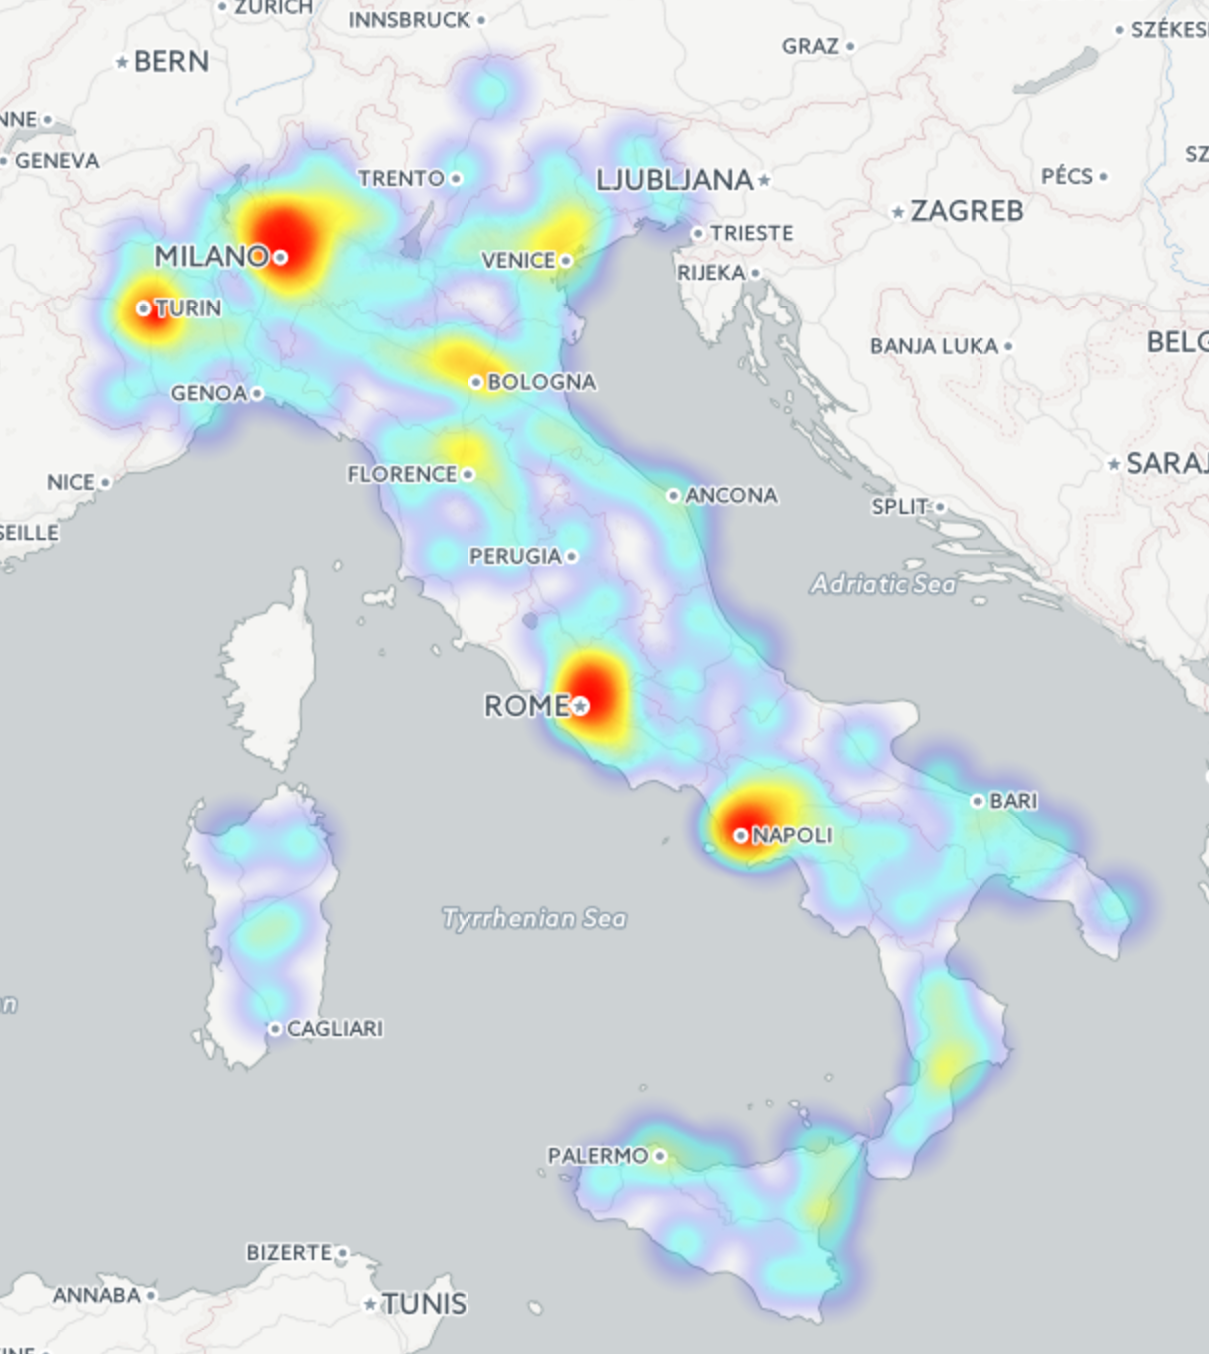
\includegraphics[width=1\linewidth]{heatmap_sottoaree.png}
\caption{Distribution of \textit{sottoaree}}
\end{figure}
As expected, a higher there is a higher concentration of \textit{sottoaree} in areas corresponding to Italy major cities, meaning that the coordinates have not been skewed by much and can be considered an useful source of information.

\begin{figure}[h]
\centering
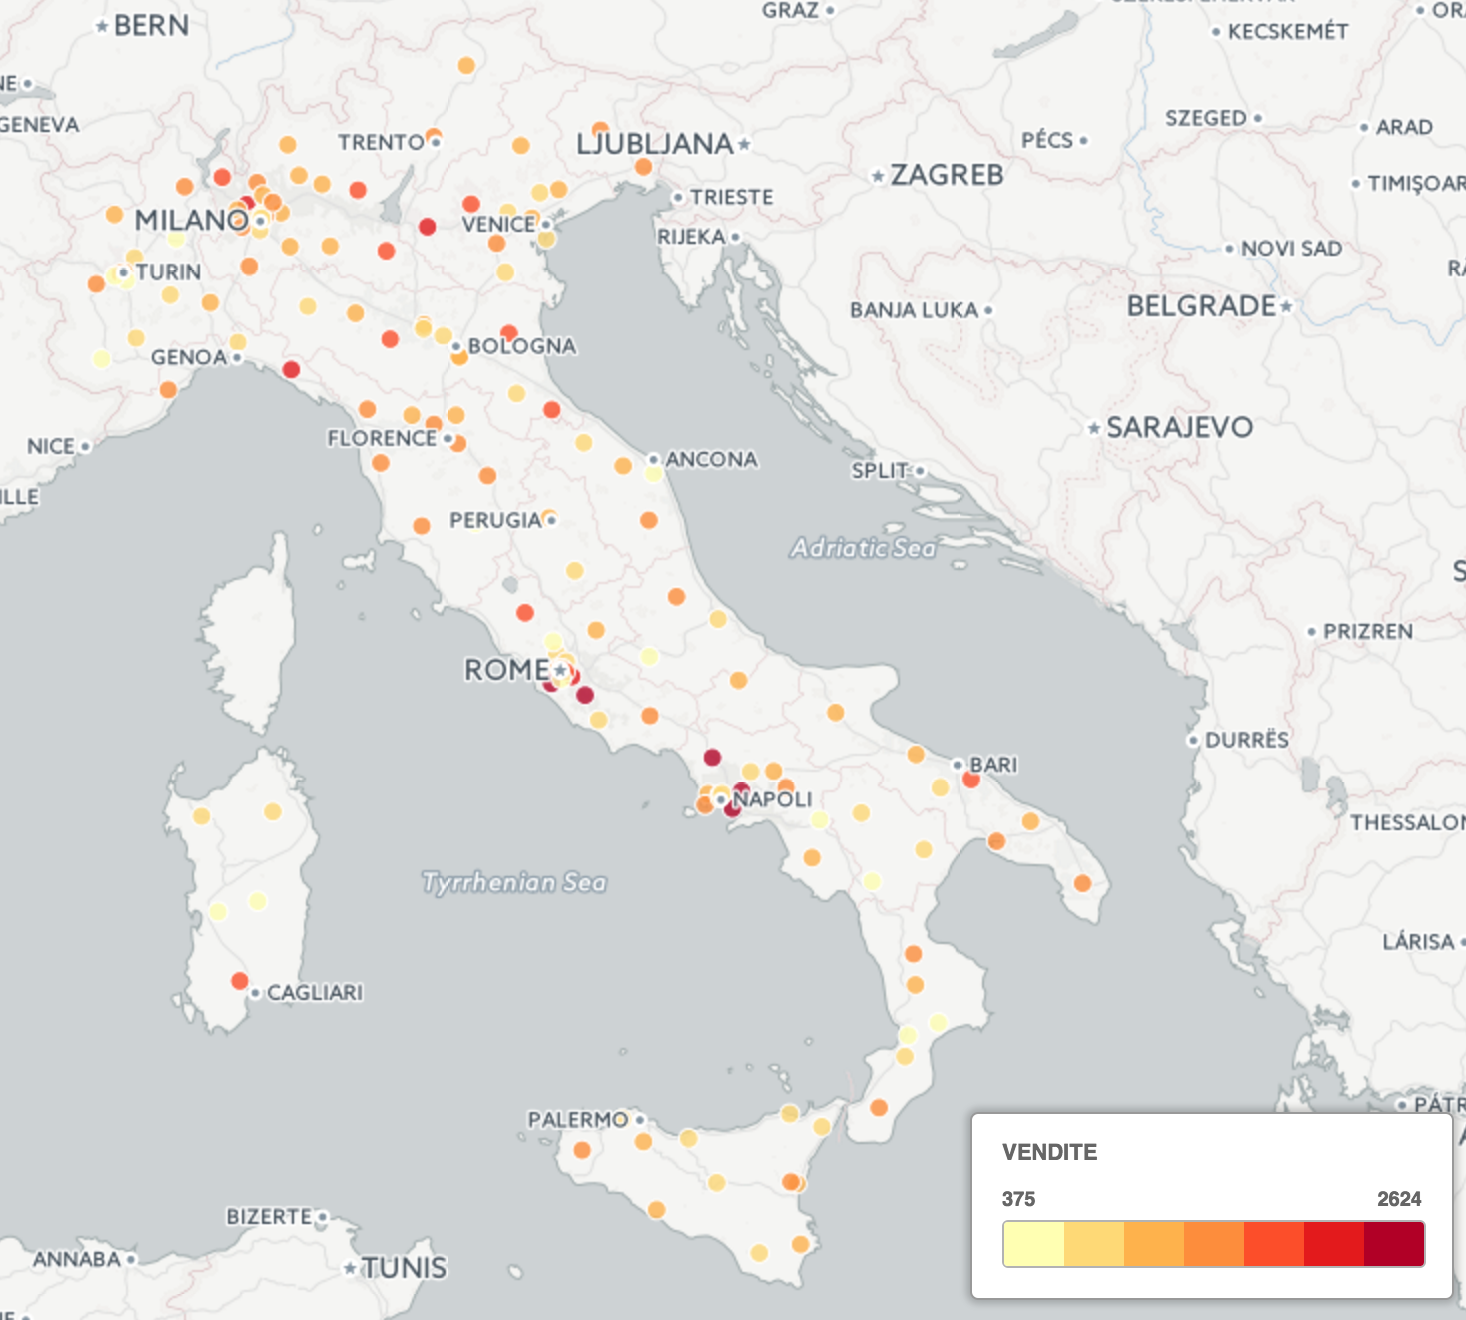
\includegraphics[width=1\linewidth]{choroplet_vendite_2016.png}
\caption{Distribution of \textit{vendite} in 2016}
\end{figure}
We plotted the data from various perspectives, to understand if there have been any non negligible variation during the 3 different years provided but apart from a general increase in numbers of \textit{sales} nothing else was detected.

\begin{wraptable}{r}{0cm}
\centering
\begin{tabular}{|c|} \hline
Day of the week\\ \hline
Day of the month\\ \hline
Day of the year\\ \hline
Month\\ \hline
Year\\ \hline
Holiday\\
\hline\end{tabular}
\caption{Data new features}
\label{table:data_new_features}
\end{wraptable}
\begin{table*}[h]
\centering
\begin{tabular}{|>{\bfseries}c c|} \hline
Region&The name of the region\\ \hline
Area&North, Centre, South\\ \hline
Island&Whether is an island or not\\ \hline
Population&Inhabitants of the city\\ \hline
MinDistance&Minimum distance to another \textit{sottoarea}\\ \hline
Density&Number of \textit{sottoarea} within 10km\\ \hline
InstructionIndex&Upper secondary education attainment rate\\ \hline
AverageIncome&The average income \\ \hline
IncomeGiniIndex&The Gini index of the distribution of the incomes\\ \hline
WorkForce&Percentage of population that can work\\ \hline
Occupation&Percentage of the work force that has a job\\
\hline\end{tabular}
\caption{Location new features}
\label{table:gps_new_features}
\end{table*}

\subsection{Feature extraction}
Next we passed to the features extraction phase.
Starting from the first csv, we expanded the \textit{Data} (see Table \ref{table:data_new_features}).

The last one, was computed based on the Italian calendar and has been a very important feature, having a high correlation with the \textit{sales}.

\newpage
From the second csv, we were able to obtain a higher number of interesting features, as we integrated and computer additional indexes from datasets extracted from the \textbf{ISTAT} data warehouse\footnote{http://dati.istat.it/}  (see Table \ref{table:gps_new_features}).



Since the first submissions, the \textit{Item Content Matrix} was first processed with the \textit{Inverse Document Frequency} function (not \textit{Term Frequency}, as it would not make sense in this case).
Changing the \textit{Inverse Document Frequency} normalization factor (e.g., from $log$ to $log2$) would not result in substantial variations in the score.

To measure the similarity between items and compute the estimated ratings, we used the \textit{Cosine Similarity} function: our goal was then to identify the shrink term $K$ that would maximise the score.
Using a trial and error approach, the highest score, \textbf{0.00544} was obtained with:\begin{equation}K=44\end{equation} 

\subsubsection{Collaborative Filtering Algorithms}
Our third approach was to implement \textit{Collaborative Filtering} algorithms: user-based and item-based.
As item-based collaborative filtering algorithms generally provide good recommendations, especially compared to the user-based ones, it was the first one to be implemented.
As a similarity function, both \textit{Cosine Similarity} and \textit{Adjusted Cosine} were used (\textit{Pearson Correlation} removes the items bias which we considered not to be too relevant).
Since the first implementations, the \textit{k-Nearest Neighbors} algorithm was used, where: 
\begin{equation}k=8\end{equation}
Additionally, \textit{Global Effects} were computed on the dataset before the collaborative filtering algorithms effectly produced the recommendations.

The \textit{Item-Based Collaborative Filtering} submissions resulted in very poor score results, pushing us to use the \textit{User-Based Collaborative Filtering} instead.
Surprisingly, still using the \textit{Consine Similarity} as user bias is removed with the \textit{Global Effects}, we obtained a better result, but still lower that the \textit{Collaborative Filtering}. 
These results suggested us the use of \textit{Hybrid} algorithms (see \ref{subsec:hybrid})

\subsubsection{Matrix Factorization and Hybrid Algorithms}
\label{subsec:hybrid}
Our last group of algorithms involved \textit{SVD} and \textit{Hybrid} algorithms. 
Expecting notable improvements in the score implementing \textit{SVD}, a relevant amount of time has been spent implementing it with different approaches. 

\textit{Matrix Factorization:} the goal was to approximate the URM as the product of two matrices by observing only the most important features.
\begin{itemize}
\item Funk's SVD: we started computing the baseline by unbiasing the URM and then iteratively minimize the prediction error of each rating, using the gradient descend, in order to learn the latent factors. Parameter used: \begin{equation}\lambda = 0.01 \;\; \gamma = 0.02 \;\;  nFactors = 100\end{equation}
\item SVD++: MATLAB natively provides a $svds(URM, k)$ function in order to get the $V'$ matrix 
\end{itemize}

\textit{Hybrid Algorithms:} we tried then to mix some of our algorithms in order to obtain better recommendations by pipelining \textit{Global Effects} and merging in the last phase: \begin{equation}\widetilde{r}_{u,i} = \alpha \cdot \widetilde{r}_{A(u,i)} + \beta \cdot \widetilde{r}_{B(u,i)}\end{equation}

Keeping the \textit{Content Based} as the $A$ algorithm, we varied $B$ with \textit{User} and \textit{Item-Based Collaborative Filtering}. 
The idea is to cope with the low number of ratings problem by computing \textit{Content Based} recommendations as a step to add some poor users profiles with meaningful ratings (i.e rating predictions for items that nobody rated before). Unfortunately the noise generated with such technique resulted in a lower score: \textbf{0.00404}.

Additionally, as \textit{SVD} resulted in very low scores, we decided to improve our existing algorithms by using \textit{SVD} and \textit{Latent Semantic Analysis} to reduce possible noise of our dataset, with little to no success.

\subsection{Evaluation}
We performed an off-line evaluation by partitioning our dataset with the \textit{Hold-Out} technique:

\begin{itemize}
  \item We took a subset of users with more than 5 positive ratings (where a positive rating is a rating greater than or equal to 8).
  \item The 80\% of the users were considered as train users while the other 20\% were test users.
  \item For each test user, 5 most unpopular items with positive rating were added to the test set, while the rest of the ratings were added to the train set.
\end{itemize}

\begin{figure}[h]
\centering
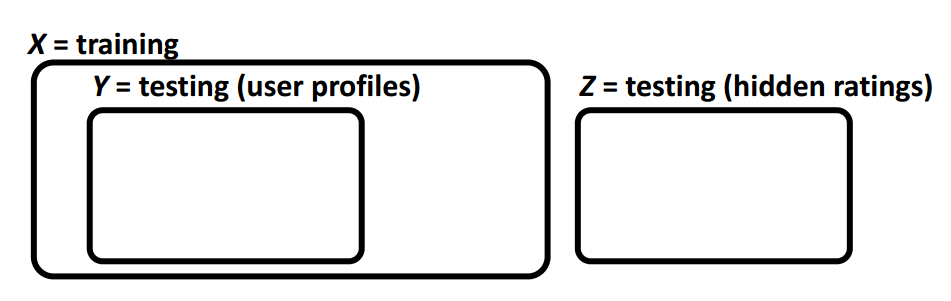
\includegraphics[width=\linewidth]{hold-out.png}
\caption{Hold-Out}
\end{figure}

We computed the \textit{RMSE(Root Mean Square Error)} in order to measure the accuracy of the predicted ratings.
\begin{equation}RMSE = \sqrt{MSE} = \sqrt{\frac{1}{\lvert T \rvert}\sum_{(u,i) \epsilon T}(r_{u,i} - \widetilde{r}_{u,i})^2}\end{equation}
where \textit{T} is the test set.

In order to keep the overfitting under control we made use of shrink terms and tried to use values that would reduce the RMSE and increasing our score on the public leader board as well.

\section{Conclusions}
%At the very end we agreed to the fact that the content based filtering techniques were the most effective due to the fact that there were very few "new items"(items without features), so we were able to provide each user a relatively good rating prediction to almost every movie in the dataset.
At the very end we agreed that the content-based recommenders were the most effective due to the fact that they do not suffer from the first-rater problem (which affects collaborative recommenders); so we were able to provide each user a relatively good rating prediction to almost every movie in the dataset.
%Content-based recommenders are capable of recommending items not yet rated by any user. As a consequence, they do not suffer from the first-rater problem, which affects collaborative recommenders which rely solely on users’ preferences to make recommendations. Therefore, until the new item is rated by a substantial number of users, the system would not be able to recommend it.

%\end{document}  % This is where a 'short' article might terminate


% That's all folks!
\end{document}
